%%%%%%%%%%%%%%%%%%%%%%%%%%%%%%%%%%%%%%
%
% This is how you write code:
%
% \begin{minted}{matlab}
% foo = [2 1 0;1 4 3;2 4.5 6];
% \end{minted}
%

% This is how you import code:
% 
% \inputminted[linenos]{matlab}{foo_bar.m}
%
 
% Most figures are imported this way:
%
% \begin{figure}
% \includegraphics[width=\textwidth]{foo_figure}
% \caption{This is a caption}
% \end{figure}

% This is a matrix:
%
% \begin{equation}
% H =
%  \left[
%  \begin{matrix}
%    1 & 2 &  3 &  4 \\ 
%    5 & 6 &  7 &  8 \\ 
%    0 & 9 & 10 & 11 \\ 
%    0 & 0 & 12 &  0
%  \end{matrix} 
% \right]
%\end{equation}
%
%%%%%%%%%%%%%%%%%%%%%%%%%%%%%%%%%%%%%%


\documentclass[00-main.tex]{subfiles}
\begin{document}




\section*{Problem One}

\subsection*{a.}

\begin{figure}[!htbp]
  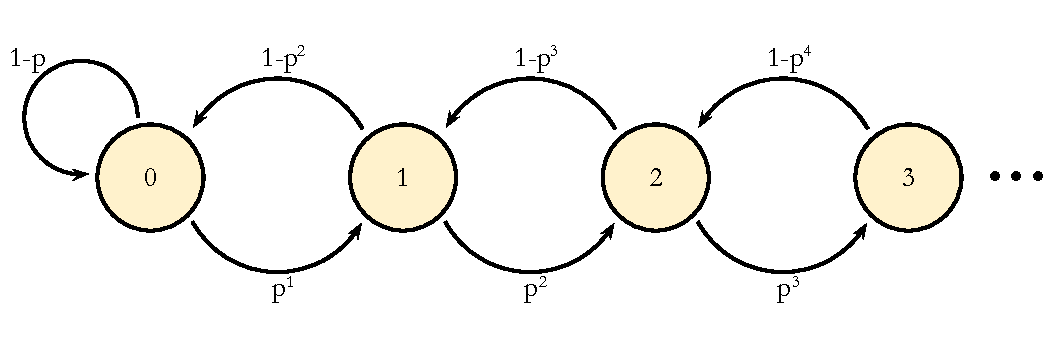
\includegraphics[width=\textwidth]{markov-chain.pdf}
  \caption{The Markov chain $P_{ij}$ illustrated as a digraph.}
  \label{markov}
\end{figure}

The Markov chain $P_{ij}$ in \cref{markov} describes a random walk. Starting in any state, you can reach any other state - i.e. all states communicate. 
Thus, $P_{ij}$ is \textbf{strongly connected}, has \textbf{one equivalence class} and is \textbf{irreducible}. 
Let $X_n$ and $X_{n+s}$ be two states such that there are $s-1$ intermediate states between them. 
To get from state $i$ to $j=i+s$ you have to visit all intermediate states at least once\footnote{Equivalently, $s$ is the minimum number of steps you must preform to make the transition from state $i$ to $i+s$}. 
Another trait of $P_{ij}$ is that with growing $i$, the probability of moving from state $i$ to $j=i+1$ diminishes exponentially, while the probability of moving back to $j'=i-1$ grows exponentially. 
Starting in state $i$, it is therefore reasonable to claim that it is always possible to return to state $i$ in a finite number of steps.
State $i$ is then said to be positive recurrent, and since positive recurrence is a class property, the whole chain is \textbf{positive recurrent}.

Starting in state $i$, let $n$ be the number that allows you to end up in state $i$ after $n$ transitions with the probability $P^{n}_{ii} > 0$. 
Let $N_i$ be the set of all such numbers for our chain. 
The greatest common divisor of the elements in $N_i$ is called the period $d$ of  state $i$.
Since $P^{n}_{00} > 0$ for any $n$, $N_i = 0, 1, 2, ...$ and so $P_{00}$ has a period of $d=1$. Since periodicity is a class property, the chain as a whole has period one. 
A Markov chain with $d=1$ is called \textbf{aperiodic}.

A positive recurrent aperiodic chain is called \textbf{ergodic}. 
Theorem 4.1 in \cite{ross} states that for an irreducible ergodic Markov chain the limit $\pi_j = \lim_{n \to \infty}P^n_{ij}$, $j \geq 0$ exists, 

\begin{equation}
\label{ergo1}
 \pi_{j} = \sum^{\infty}_{i = 0} \pi_{i} P_{ij}
\end{equation}

and 

\begin{equation}
\label{ergo2}
 \sum^{\infty}_{j = 0} \pi_{j} = 1.
\end{equation}

In this case \cref{ergo1} becomes

\begin{align}
\label{pi_i}
  \pi_{i} = \left\{ 
  \begin{array}{l l l}
    \pi_{i-1} P_{i-1,i} + \pi_{i+1} P_{i+1,i} &= \pi_{i-1} p^i + \pi_{i+1} (1-p^{i+2}) & \quad i>0\\
    \pi_{i} P_{i,i} + \pi_{i+1} P_{i+1,i} &= \pi_{0}(1-p) + \pi_{1}(1-p) & \quad i=0\\
  \end{array} \right.
\end{align}

The $\pi$'s are called the limiting probabilities that the process will be in state $i$ at time $n$, and it can be shown that $\pi_i$ also equals the long-run proportion of time that the process will be in state $i$. Below the limiting probabilities are calculated for the first 3 states.

\begin{align*}
\pi_1 =  \frac{p}{1-p^2} \pi_0; \quad
\pi_2 =  \frac{p^2}{1-p^3} \pi_1; \quad
\pi_3 =  \frac{p^3}{1-p^4} \pi_2
\end{align*}

By induction this yields the general formula (recurrence relation)

\begin{equation}
\label{pi_i}
\begin{aligned}
\pi_{i+1} =  \frac{p^{i+1}}{1-p^{i+2}} \pi_{i}
  &= \frac{p^{i+1}p^{i}p^{i-1} \cdots p^{2} p^{1}}{(1-p^{i+2})(1-p^{i+1})(1-p^{i}) \cdots (1-p^{3})(1-p^{2})} \pi_{0} \\
  &= \frac{p^{1+2+...+(i-1)+i+(i+1)}}{\prod_{i=2}^{k=i+2} (1-p^{k})} \pi_{0} 
  = \frac{p^{\frac{1}{2}(i+1)(i+2)}}{\prod_{i=2}^{k=i+2} (1-p^{k})} \pi_{0} \\
  \text{or, equivalently,} \\
\pi_{i} &= \pi_{0} \cdot \prod_{k=1}^{k=i+1}  \frac{p^k}{1-p^{k+1}}
 \end{aligned}
\end{equation}

Now \cref{ergo2} becomes

\begin{equation}
\label{pi_start}
\begin{aligned}
\sum_i \pi_{i} &= \pi_{0} \left(1 + \sum_i \cdot \prod_{k=1}^{k=i+1}  \frac{p^k}{1-p^{k+1}} \right) = 1 \\
\implies
\pi_{0} &= \left(1 + \sum_i \cdot \prod_{k=1}^{k=i+1}  \frac{p^k}{1-p^{k+1}} \right)^{-1}
\end{aligned}
\end{equation}

Substituting \cref{pi_start} into \cref{pi_i} gives an expression for the limiting probabilities

\begin{equation}
\pi_{i} = \frac{\prod_{k=1}^{k=i+1}  \frac{p^k}{1-p^{k+1}}}{1 + \sum_i \cdot \prod_{k=1}^{k=i+1}  \frac{p^k}{1-p^{k+1}}} 
\end{equation}


The distribution is positive so the limiting probabilities exist and the states are indeed positive recurrent. 


\subsection*{b.}

Let the set $\xi$ contain the first 10 states, and let $T_i$ be the time spent to reach state 10, starting in state $X_0 = i \in \xi$. 


\begin{equation}
\label{exp_time}
\begin{aligned}
 \mu_i &= E[T_i] \\
       &= E[T_{i}|X_1 = i-1]P(X_1=i-1) + E[T_{i}|X_1 = i+1]P(X_1=i+1) \\
       &= ( 1+E[T_{i-1}] )( 1-p^{i+1} ) + ( 1+E[T_{i+1}] )p^{i+1} \\
       &= 1 + \mu_{i-1} + ( \mu_{i+1} - \mu_{i-1} )p^{i+1}
\end{aligned}
\end{equation}

Note the special cases for $\mu_0 = 1 + \mu_0 + (\mu_1 - \mu_0)p$, and $\mu_9 = 1 + \mu_8(1-p^{10})$

\cref{exp_time} constitutes a set of 10 equations that can be solved with \textsc{matlab}. 
In table <TABLE> the solutions are listed for $p=0.75$ and $p=0.90$.

% Table
% here

The exponetial decay for the probabilities for moving on to the next state  clearly manifests itself for the case of $p=0.75$; no matter what state you start in, you'll have to wait for a very long time to reach state 10. The transition from state 9 to 10 is taking very long time compared to the other one-step transitions. 


\subsection*{c.}

The probability for ever reaching state 100 is 1, no matter what state you start in, since all limiting probabilities are positive. If you start in state $X_0<100$, you will have to wait for a very long time to reach state 100, and if $X_0>100$ you will only have to wait close to $X_0 - 100$ steps (at least if not $p \approx 1$).


\subsection*{d.}

\textsc{matlab} is here used to illustrate some random walks.

\begin{minted}{matlab}
hold on;
%%% A ten-step illustrated random walks, p=0.90
% Starting in state 0
plot(randwalk(20,0,0.9), "1", \
randwalk(20,0,0.9), "2", randwalk(20,0,0.9), "3" )
% Starting in state 5
plot(randwalk(20,5,0.9), "1", \
randwalk(20,5,0.9), "2", randwalk(20,5,0.9), "3" )
% Starting in state 9
plot(randwalk(20,9,0.9), "1", \
randwalk(20,9,0.9), "2", randwalk(20,9,0.9), "3" )

%%% p=0.75
% Starting in state 0
plot(randwalk(20,0,0.75), "1", \
randwalk(20,0,0.75), "2", randwalk(20,0,0.75), "3" )
% Starting in state 5
plot(randwalk(20,5,0.75), "1", \
randwalk(20,5,0.75), "2", randwalk(20,5,0.75), "3" )
% Starting in state 9
plot(randwalk(20,9,0.75), "1", \
randwalk(20,9,0.75), "2", randwalk(20,9,0.75), "3" )

\end{minted}

Notice the difference between $p=0.90$ and $p=0.75$ in \cref{randwalk1,randwalk2}. Walking with $p=0.75$ does indeed pull you down towards state 0.
\begin{figure}[!htbp]
  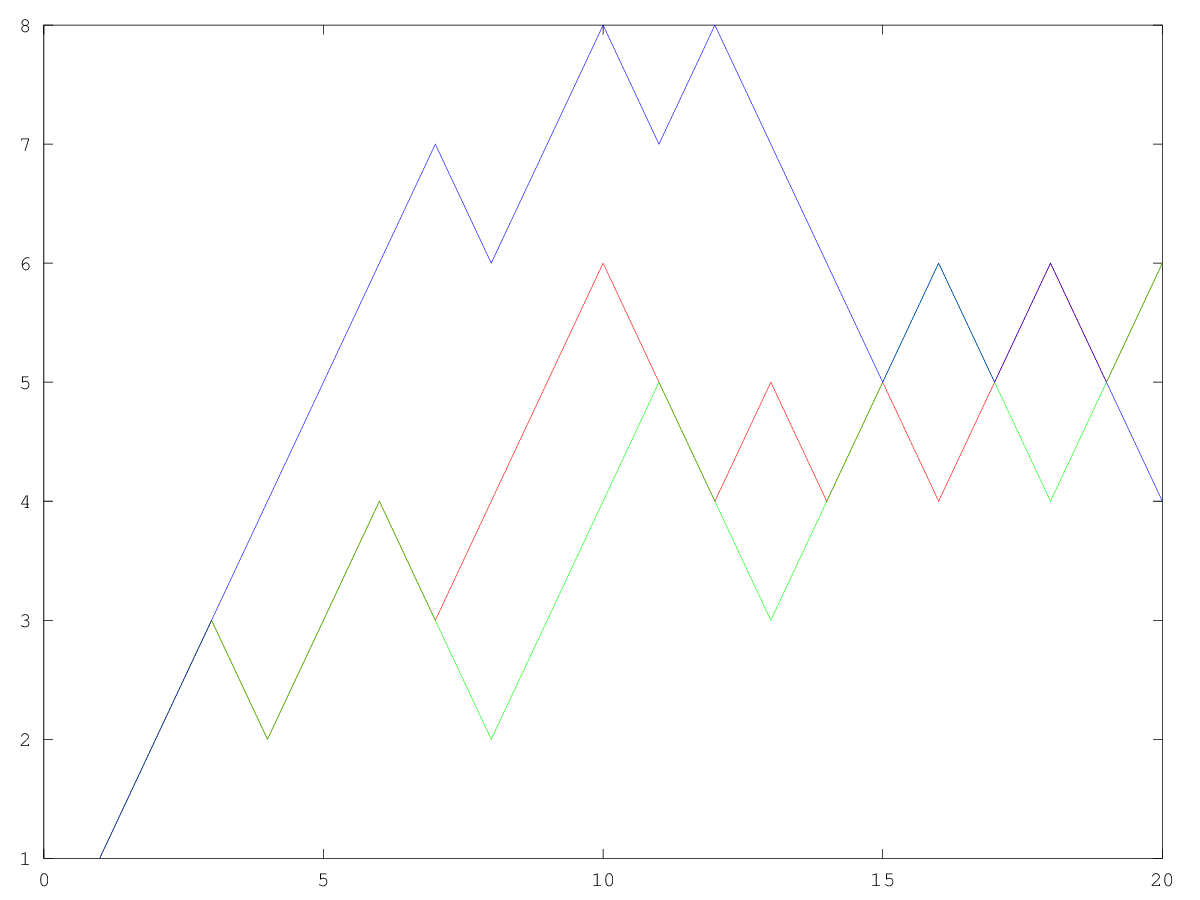
\includegraphics[width=\textwidth/2]{randwalk0.png}
  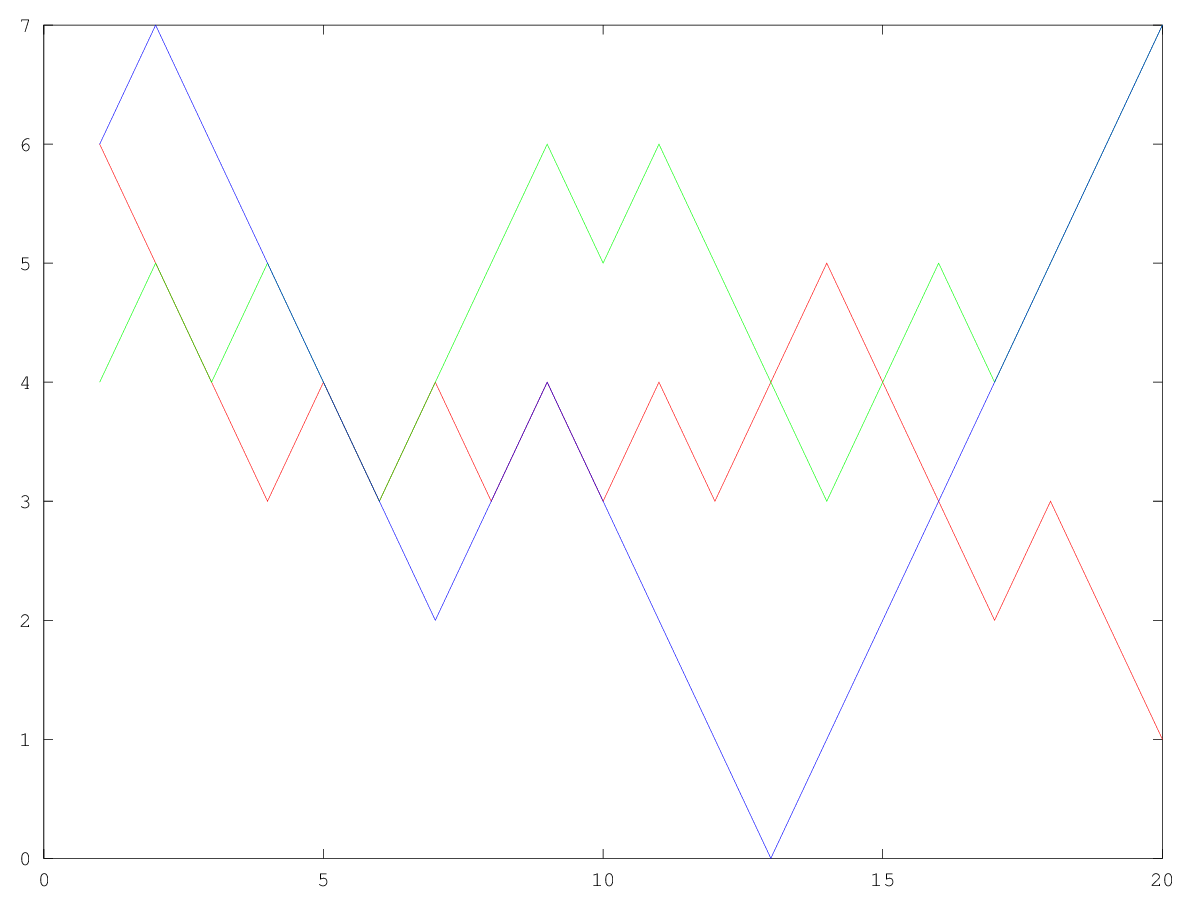
\includegraphics[width=\textwidth/2]{randwalk5.png}
  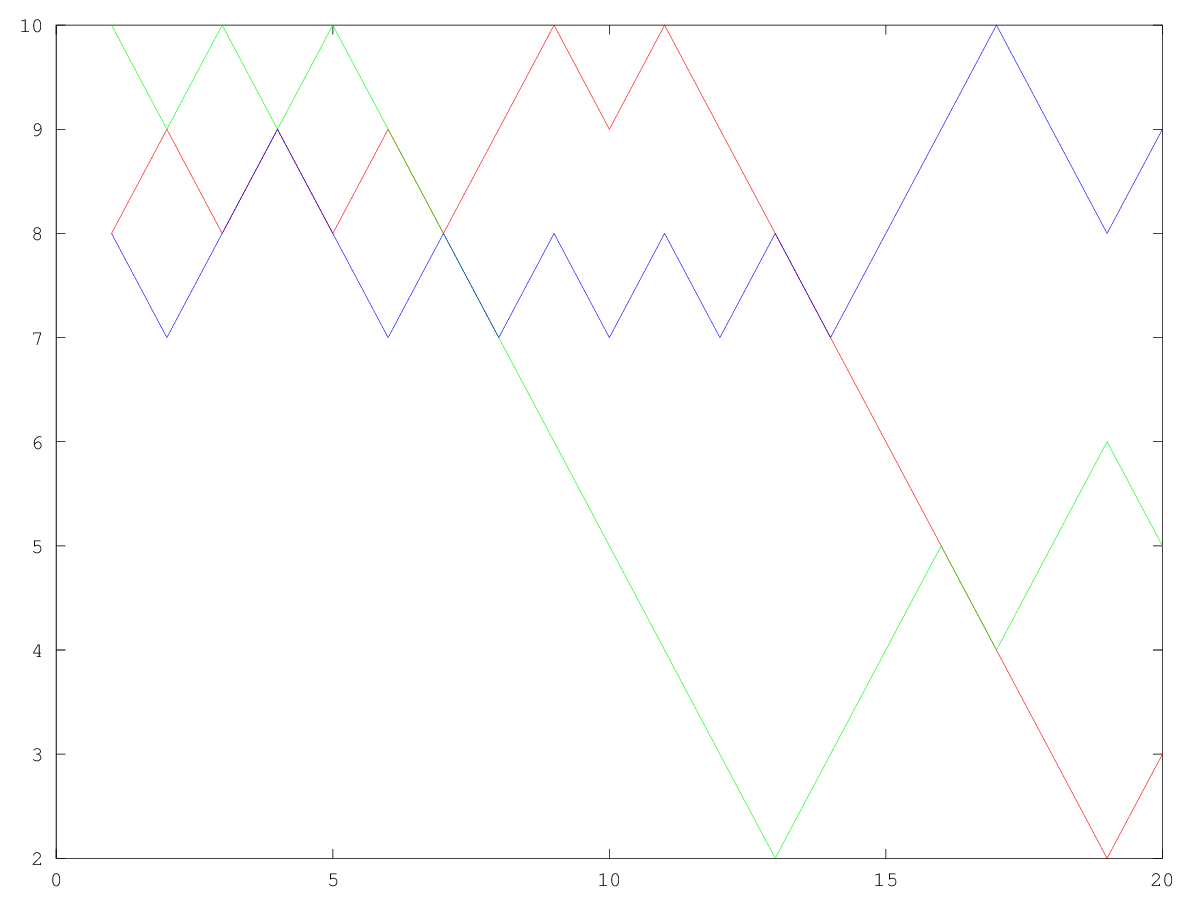
\includegraphics[width=\textwidth/1]{randwalk9.png}
  \caption{A 20-step random walk w. $p=0.90$ starting with state 0, 5 and 9, respectively.}
  \label{randwalk1}
\end{figure}


\begin{figure}[!htbp]
  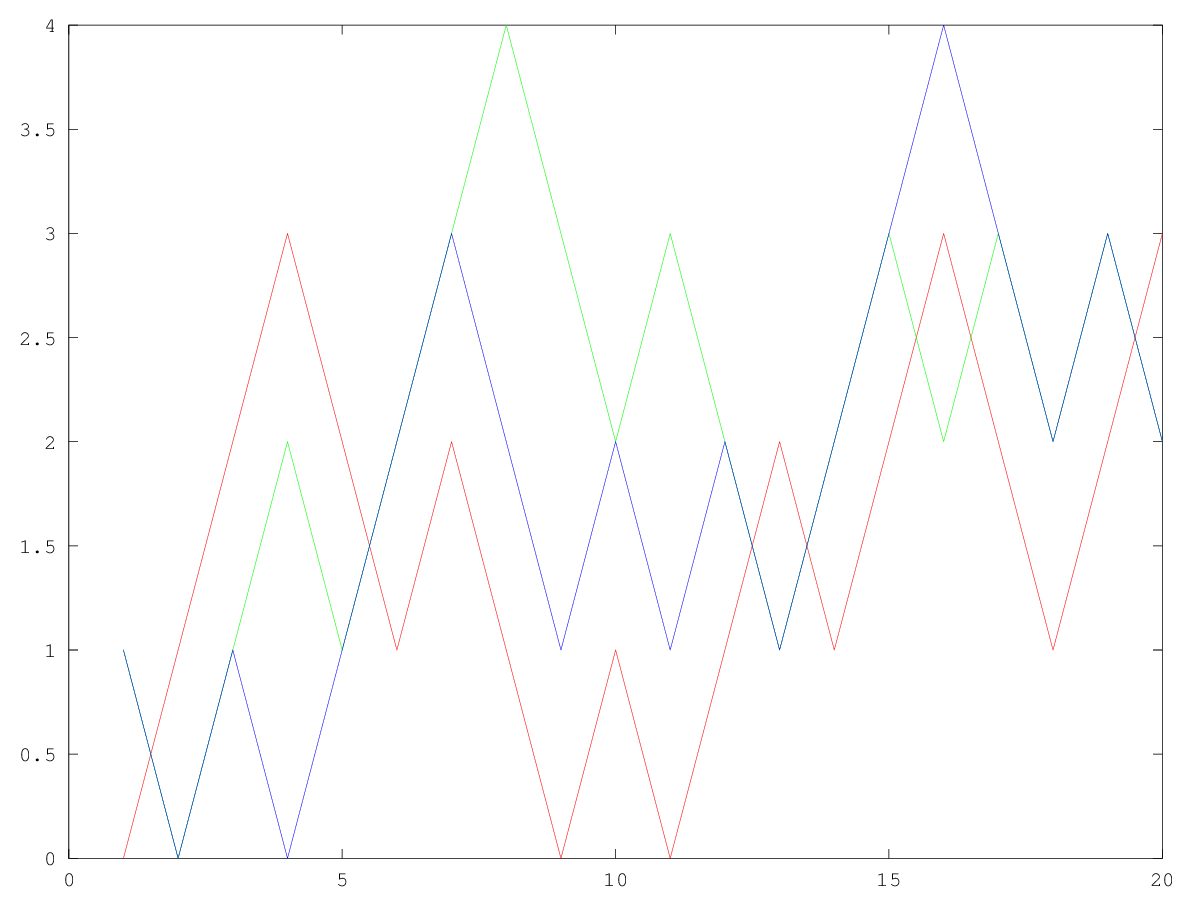
\includegraphics[width=\textwidth/2]{randwalk0_75.png}
  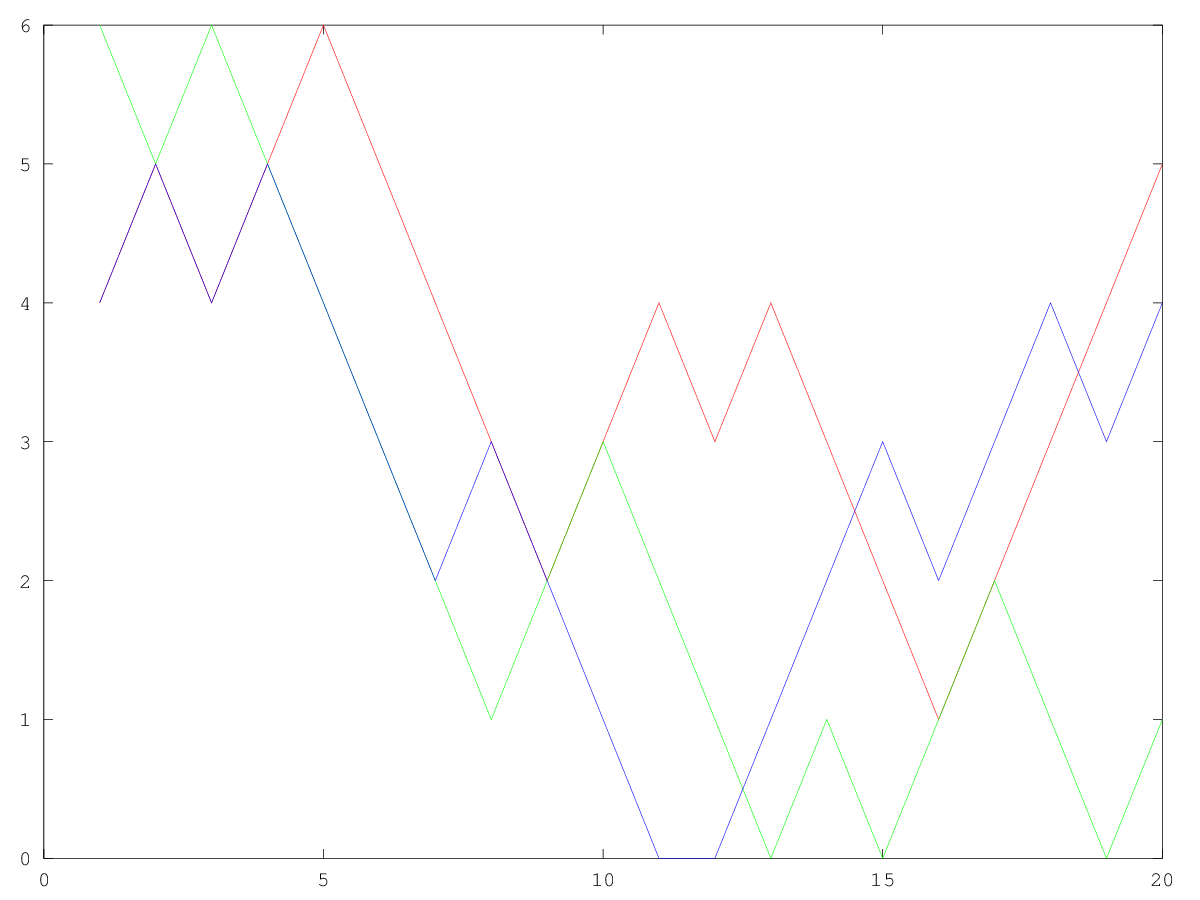
\includegraphics[width=\textwidth/2]{randwalk5_75.png}
  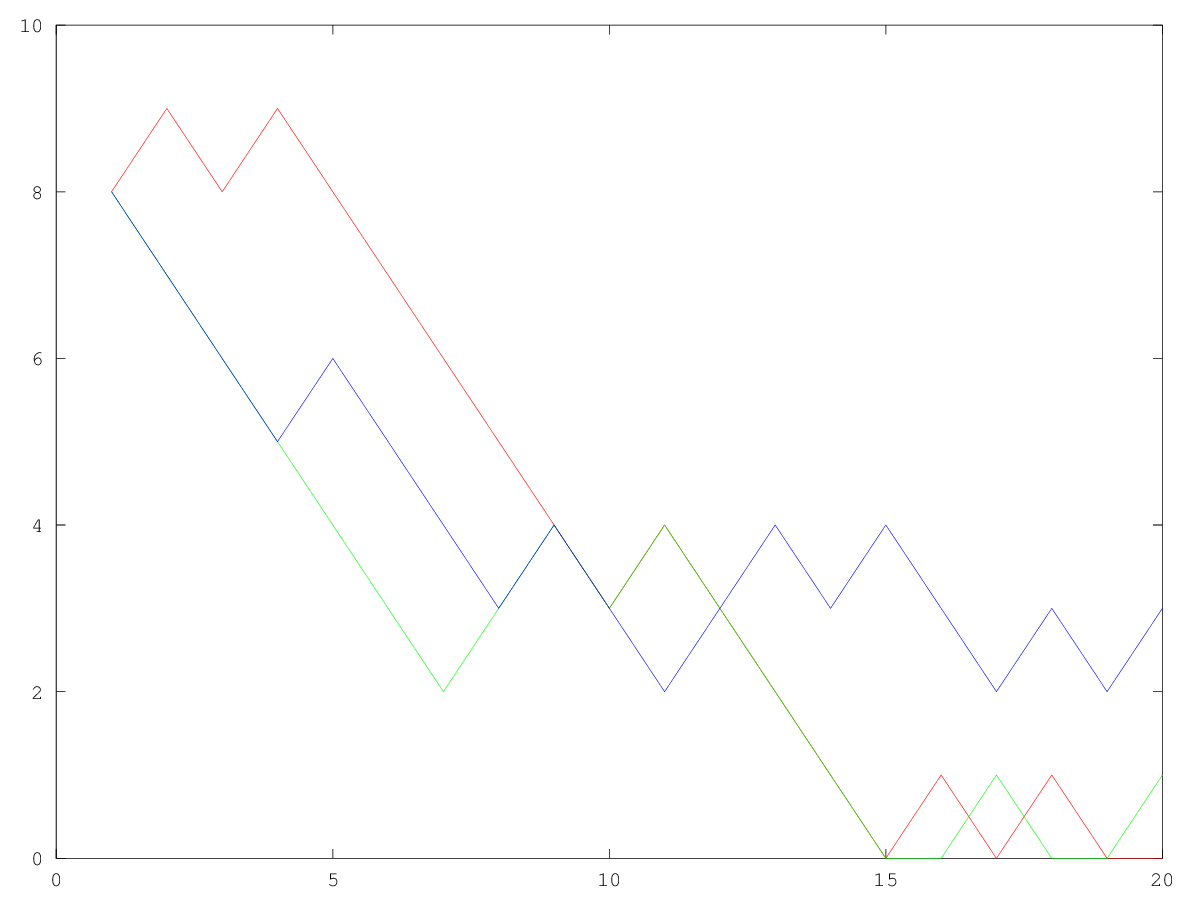
\includegraphics[width=\textwidth/1]{randwalk9_75.png}
  \caption{A 20-step random walk w. $p=75$ starting with state 0, 5 and 9, respectively.}
  \label{randwalk2}
\end{figure}

\begin{table}[!htbp]
\centering
\begin{tabular}{ccccc}
  \hline
  \noalign{\smallskip}
  j & $\pi_j$ & $\bar{\pi_j}$ & \multicolumn{2}{c|}{C.I.} \\
  \hline
  \noalign{\smallskip}
  0   & .1669 & 0.1677 & .1666  & .1688  \\
  1   & .2861 & 0.2867 & .2856  & .2877  \\
  2   & .2789  & .2774 & .2767  & .2782  \\
  3   & .1718  & .1708 & .1699  & .1717  \\
  4   & .0713  & .0714 & .0706  & .0721  \\
  5   & .0206  & .0205 & .0201  & .0210  \\
  6   & .0042  & .0042 & .0040  & .0044  \\
  7   & .0006  & .0006 & .0005  & .0006  \\
  8   & .0001  & .0001 & .0000  & .0001  \\
  9   &   0    &   0   &    0   &   0    \\
  10  &   0    &   0   &    0   &   0    \\
\hline
\end{tabular}
\caption{The analytical and simulated limiting probabilities for the first 11 states are shown together with the corresponding 95\% confidence interval.}
\label{lim_p}
\end{table}


\end{document}
